% =====================================================================
%  Status-by-step presentation (Beamer, single-file)
%  Mirrors the proposal deck's 7-step roadmap: what's done, what broke, how we fixed it.
%  Build:  report/build.sh report/presentation   (Tectonic + Ghostscript-normalise)
% =====================================================================
\documentclass[aspectratio=169,11pt]{beamer}
\usetheme{default}
\setbeamertemplate{navigation symbols}{}
\setbeamertemplate{footline}[frame number]
\setbeamertemplate{itemize items}[circle]

\usepackage{amsmath,amssymb}
\usepackage{booktabs}
\usepackage{tikz}
\usetikzlibrary{positioning,arrows.meta,calc}

\definecolor{navy}{RGB}{30,64,124}
\definecolor{forest}{RGB}{34,120,60}
\definecolor{burnt}{RGB}{214,104,26}
\definecolor{plum}{RGB}{140,55,135}
\setbeamercolor{structure}{fg=navy}
\setbeamercolor{frametitle}{fg=navy}
\setbeamerfont{frametitle}{series=\bfseries}

% status badges + a plain "snag -> fix" block
\newcommand{\badge}[2]{\colorbox{#1!20}{\small\color{#1}\textbf{#2}}}
\newcommand{\dn}{\badge{forest}{DONE}}
\newcommand{\bt}{\badge{navy}{BUILT}}
\newcommand{\nx}{\badge{burnt}{NEXT}}
\newcommand{\snag}[2]{\textbf{\color{burnt}Snag:} #1\; \textbf{\color{forest}Fix:} #2}

\title[Status by step]{Predicting the Zero-Shot Transfer of a Promptable Video Tracker}
\subtitle{Status by step --- what's done, what broke, and how we fixed it}
\author{Kostiantyn Boiar}
\institute{MSc Dissertation \,\textbullet\, University of Glasgow\\[2pt]
\small Supervisor: Dr Marwa Mahmoud}
\date{\today}

\begin{document}

% ---------------------------------------------------------------- title
\begin{frame}[plain]\titlepage\end{frame}

% ------------------------------------------------------------ overview
\begin{frame}{Progress against the seven-step plan}
  \centering
  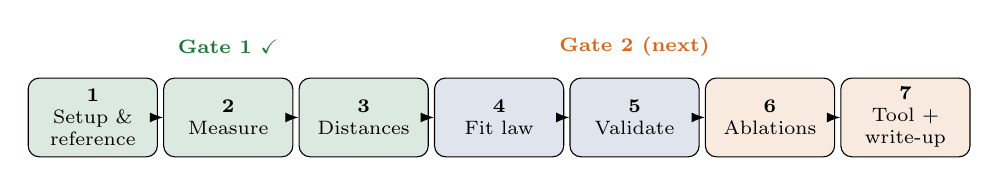
\begin{tikzpicture}[>=Latex, x=1.72cm,
    st/.style={draw,rounded corners,align=center,font=\scriptsize,inner sep=2pt,
               text width=1.5cm,minimum height=1.0cm}]
    \node[st,fill=forest!16] (s1) at (0,0) {\textbf{1}\\Setup \&\\reference};
    \node[st,fill=forest!16] (s2) at (1,0) {\textbf{2}\\Measure};
    \node[st,fill=forest!16] (s3) at (2,0) {\textbf{3}\\Distances};
    \node[st,fill=navy!14]   (s4) at (3,0) {\textbf{4}\\Fit law};
    \node[st,fill=navy!14]   (s5) at (4,0) {\textbf{5}\\Validate};
    \node[st,fill=burnt!14]  (s6) at (5,0) {\textbf{6}\\Ablations};
    \node[st,fill=burnt!14]  (s7) at (6,0) {\textbf{7}\\Tool +\\write-up};
    \foreach \a/\b in {s1/s2,s2/s3,s3/s4,s4/s5,s5/s6,s6/s7} \draw[->] (\a)--(\b);
    \node[forest,font=\scriptsize\bfseries] at ($(s2)+(0,0.9)$) {Gate 1 \checkmark};
    \node[burnt,font=\scriptsize\bfseries]  at ($(s5)+(0,0.9)$) {Gate 2 (next)};
  \end{tikzpicture}
  \vspace{0.8em}

  \centering \dn\ done \& validated \quad \bt\ code built, awaiting the run \quad \nx\ not started
  \vspace{0.4em}

  \footnotesize The measurement half (steps 1--3) is finished and \textbf{Gate 1 is passed}; the modelling
  code (steps 4--5) is written and unit-tested, waiting only for the real run.
\end{frame}

% ------------------------------------------------------------ step 1
\begin{frame}{Step 1 --- Setup \& the leakage firewall \hfill \dn}
  \textbf{What we did}
  \begin{itemize}
    \item Pulled SA-FARI --- gated outlines (Hugging Face) $+$ public frames (Google Cloud).
    \item Froze the ``seen'' reference and built the \textbf{leakage firewall}: distances only ever see the
          reference side (with an automated test that a species can't fake ``distance 0'' to itself).
  \end{itemize}
  \vspace{0.3em}
  \begin{block}{Snags \& fixes}\footnotesize
    \begin{itemize}
      \item \snag{the split separates \emph{places} but reuses \emph{species} --- not what we assumed.}
            {re-planned as \textbf{two} experiments (hide a species / hide a place); the frozen model lets
             us re-slice freely.}
      \item \snag{downloading the labels failed with a permissions error (a Hugging Face transfer quirk).}
            {switched off the new transfer backend --- plain download works.}
    \end{itemize}
  \end{block}
\end{frame}

% ------------------------------------------------------------ step 2
\begin{frame}{Step 2 --- Measure: frozen SAM\,3 $\to$ official scorer \hfill \dn}
  \textbf{What we did}
  \begin{itemize}
    \item Ran frozen SAM\,3 over the \emph{whole} test split and scored it with the \textbf{official}
          evaluator, aggregated to one row per (species, place, year).
  \end{itemize}
  \vspace{0.3em}
  \begin{block}{Result --- and why we trust it}\footnotesize
    \textbf{pHOTA 0.65 \; / \; pDetA 0.52 (detection) \; / \; pAssA 0.81 (association).}
    \vspace{0.3em}
    Three independent checks: the numbers are \textbf{internally consistent}; they \textbf{reproduce the
    published SAM\,3 figures} (our zero-shot $+$ the paper's fine-tuning gain lands on their fine-tuned
    result); and the model essentially \textbf{never invents} an animal that isn't there.
    \textcolor{forest}{\textbf{Gate 1 passed.}}
  \end{block}
\end{frame}

% ------------------------------------------------------------ step 3
\begin{frame}{Step 3 --- The four distances \& the feature table \hfill \dn\;/\;\bt}
  \textbf{What we did}
  \begin{itemize}
    \item Built \& sanity-checked all four label-free distances (taxonomic, visual, environment,
          temporal) on real data. \dn
    \item Built the assembler that joins distances $+$ scores into one modelling table
          (\texttt{features.parquet}); unit-tested. \bt\ (awaits the GPU features run.)
  \end{itemize}
  \vspace{0.3em}
  \begin{block}{Snag \& fix --- speed}\footnotesize
    \snag{on Colab, saving thousands of tiny frames to Google Drive was crippling ($\sim$43\,s per clip).}
    {downloaded frames \textbf{in parallel} to the machine's own fast disk --- $\sim$4\,s per clip, an
     $\sim$10$\times$ speed-up.}
  \end{block}
\end{frame}

% ------------------------------------------------------------ steps 4-5
\begin{frame}{Steps 4 \& 5 --- Fit the law \& validate \hfill \bt}
  \begin{itemize}
    \item \textbf{Step 4 --- fit the law.} The model (predict \texttt{pDetA}/\texttt{pAssA} from the
          distances, weighted by how much data backs each score) $+$ the ``which factor matters?''
          breakdown are \textbf{written and unit-tested on synthetic data}. \bt
    \item \textbf{Step 5 --- out-of-sample check.} Hide whole species / whole places and predict them from
          distance alone, with honest error bars --- \textbf{coded and tested}. \bt
  \end{itemize}
  \vspace{0.3em}
  \begin{block}{}
    \centering\footnotesize No snags yet --- these run on plain CPU and are waiting only for the real
    \texttt{features.parquet}. Running them is \textbf{Gate 2}: \emph{does distance really predict a
    held-out species or place?}
  \end{block}
\end{frame}

% ------------------------------------------------------------ steps 6-7
\begin{frame}{Steps 6 \& 7 --- Ablations \& the reliability tool \hfill \nx}
  \begin{itemize}
    \item \textbf{Step 6 --- ablations \& robustness:} drop each distance to see what it contributes; re-run
          under alternative choices to confirm the findings hold. \nx
    \item \textbf{Step 7 --- the deployment tool \& write-up:} a new (species, place) $\to$ a predicted
          score $+$ a confidence interval; then the dissertation. \nx
  \end{itemize}
  \vspace{0.4em}
  \begin{block}{}
    \centering\footnotesize Deliberately deferred until Gate 2 confirms a real signal --- no point polishing
    a tool before we know the law holds.
  \end{block}
\end{frame}

% ------------------------------------------------------------ environment
\begin{frame}{The biggest practical hurdle --- the environment}
  \begin{block}{Snag --- Colab kept fighting us}\footnotesize
    No proper SSH/command-line; it \textbf{slept overnight and stopped} mid-run; each fresh session
    \textbf{re-downloaded the 3.4\,GB model} and hit the permissions error again; and the GPU limits were
    too tight for a full run.
  \end{block}
  \vspace{0.3em}
  \begin{block}{Fix --- move to a machine we control}\footnotesize
    A \textbf{RunPod GPU over SSH} with a \textbf{persistent disk}: no sleep, no re-downloads, resumable
    long runs, and I can drive the whole pipeline start-to-finish. (Setup captured in a repo runbook.)
  \end{block}
\end{frame}

% ------------------------------------------------------------ closing
\begin{frame}{Where we stand}
  \begin{block}{}
    \centering The \textbf{measurement half is done and validated} (Gate 1) --- and it reproduces the
    published SAM\,3 numbers. Every snag along the way is now fixed and captured in code.
  \end{block}
  \vspace{0.5em}
  \centering
  \textbf{Next action:} run the distances $+$ fit the law on the SSH machine $\to$ \textcolor{burnt}{Gate 2}.
  \vspace{0.6em}

  {\small\color{navy}\textbf{Thank you --- questions welcome.}}
\end{frame}

\end{document}
